%%%%%%%%%%%%%%%%%%%%%%%%%%%%%%%%%%%%%%%%%%%%%%%%%%%%%%%
% NOTAS TEORIA DE TRANSPORTE OPTIMO
%
% Contains ?? figures. 
% File started: ??
% First circulated version: ??
% Last version:
% Last modification: -
%%%%%%%%%%%%%%%%%%%%%%%%%%%%%%%%%%%%%%%%%%%%%%%%%%%%%%%

\documentclass[11pt,a4paper]{amsart}
\usepackage{xr-hyper}
\newcounter{chapter}
\usepackage{fancyhdr}
\usepackage{geometry} \geometry{top=2cm,bottom=2.5cm,left=2.5cm,right=2.5cm}

\usepackage{amssymb}
\usepackage{hyperref}
\usepackage{listings}
\usepackage{mathtools}
\usepackage{enumitem}

% Fuzz -------------------------------------------------------------------
% Line spacing -----------------------------------------------------------

%%%%%%%%%fin pegada%%%%%%%%%%%%%%%%%%5

\usepackage[T1]{fontenc}
\usepackage[spanish]{babel}
\usepackage{graphicx}
\usepackage{tikz}
\usetikzlibrary{babel}



\parskip 3pt

%%
%% OPERADORES
%%
\renewcommand{\Re}{\operatorname{Re}}
\newcommand{\tr}{\operatorname{tr}}
\newcommand{\id}{\operatorname{id}}
\def\div{\operatorname {\mathrm{div}}}
\def\Dom{\operatorname {\mathrm{Dom}}}
\def\argmin{\operatorname {\mathrm{arg\, min}}}
\def\argmax{\operatorname {\mathrm{arg\, max}}}
\def\gen{\operatorname {\mathrm{gen}}}
\def\Im{\operatorname {\mathrm{Im}}}
\def\Nu{\operatorname {\mathrm{Nu}}}
\def\sop{\operatorname {\mathrm{sop}}}
\def\diam{\operatorname {\mathrm{diam}}}
\def\dist{\operatorname {\mathrm{dist}}}
\def\var{\operatorname {\mathrm{Var}}}
\def\codim{\operatorname {\mathrm{codim}}}
\def\pint{\operatorname {--\!\!\!\!\!\int\!\!\!\!\!--}}

%%
%% EPSILON
%%
\newcommand{\ve}{\varepsilon}

%%
%% LETRAS MATHBB
%%
\newcommand{\R}{{\mathbb R}}
\newcommand{\Z}{{\mathbb Z}}
\newcommand{\C}{{\mathbb C}}
\newcommand{\Q}{{\mathbb Q}}
\newcommand{\N}{{\mathbb N}}
\newcommand{\E}{{\mathbb E}}
\newcommand{\V}{{\mathbb V}}
\renewcommand{\P}{{\mathbb P}}
\newcommand{\II}{{\mathbb I}}
\newcommand{\OO}{{\mathbb O}}
\newcommand{\Sb}{{\mathbb S}}
\newcommand{\Tb}{{\mathbb T}}

%%
%% LETRAS CALIFGRAFICAS
%%
\newcommand{\F}{{\mathcal F}}
\newcommand{\Hc}{{\mathcal H}}
\newcommand{\Tc}{{\mathcal T}}
\newcommand{\Ec}{{\mathcal E}}
\newcommand{\Vc}{{\mathcal V}}
\newcommand{\A}{{\mathcal A}}
\newcommand{\J}{{\mathcal J}}
\newcommand{\G}{{\mathcal G}}
\newcommand{\U}{{\mathcal U}}
\newcommand{\B}{{\mathcal B}}
\newcommand{\Sw}{{\mathcal S}}
\newcommand{\D}{{\mathcal D}}
\newcommand{\M}{{\mathcal M}}
\newcommand{\LL}{{\mathcal L}}

%%
%% LETRAS MATHBF
%%
\newcommand{\ab}{{\mathbf a}}
\newcommand{\bb}{{\mathbf b}}
\newcommand{\cc}{{\mathbf c}}
\newcommand{\ee}{{\mathbf e}}
\newcommand{\ff}{{\mathbf f}}
\newcommand{\gb}{{\mathbf g}}
\newcommand{\hh}{{\mathbf h}}
\newcommand{\n}{{\mathbf n}}
\newcommand{\mm}{{\mathbf m}}
\newcommand{\pp}{{\mathbf p}}
\newcommand{\qq}{{\mathbf q}}
\newcommand{\sbf}{{\mathbf s}}
\newcommand{\tb}{{\mathbf t}}
\newcommand{\uu}{{\mathbf u}}
\newcommand{\vv}{{\mathbf v}}
\newcommand{\ww}{{\mathbf w}}
\newcommand{\xx}{{\mathbf x}}
\newcommand{\yy}{{\mathbf y}}
\newcommand{\zz}{{\mathbf z}}
\newcommand{\I}{{\mathbf 1}}
\newcommand{\Pb}{{\mathbf P}}
\newcommand{\XX}{{\mathbf X}}
\newcommand{\YY}{{\mathbf Y}}

%%
%% LETRAS MATHFRAK
%%

\newcommand{\Gk}{{\mathfrak G}}


%%
%% TEOREMAS
%%
\newtheorem{teo}{Teorema}[section]
\newtheorem{lema}[teo]{Lema}
\newtheorem{prop}[teo]{Proposición}
\newtheorem{cor}[teo]{Corolario}

%%
%% REMARK
%%
\theoremstyle{remark}
\newtheorem{obs}[teo]{Observación}

%%
%% DEFINICION
%%
\theoremstyle{definition}
\newtheorem{defi}[teo]{Definición}
\newtheorem{ejem}[teo]{Ejemplo}
\newtheorem{ejer}[teo]{Ejercicio}
\newtheorem{nota}[teo]{Notación}
\newtheorem{ejercicio}{Ejercicio}[chapter]


%%
%% NUMERACION
%%
\numberwithin{subsection}{section}
\numberwithin{equation}{section}

%%
%% TITULO
%%


\vfuzz7pt \hfuzz7pt
\externaldocument[N-]{../notas/Notas-TO}
\newcommand{\encabezado}[1]{%
\noindent 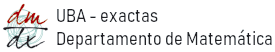
\includegraphics[scale=2.1]{logo-dm-wide.png} \hskip 9.5cm

\includegraphics[scale=0.08]{logo-exactas-uba.jpg}
\smallskip
\usefont{T1}{phv}{m}{n}
\begin{center}{\Large\sc Teoría de Transporte Óptimo}\end{center}
\bigskip
\noindent{\sc #1}\\[-0.4cm]
\hrule
\normalfont}
\newcommand{\cuadernolink}[2]{\noindent\textbf{Cuaderno:} \emph{#1} (\href{https://colab.research.google.com/github/jfbonder/transporte-optimo/blob/main/cuadernos/#2}{abrir en Colab}).\par\medskip}

\begin{document}
\renewcommand{\thechapter}{8}
\encabezado{Práctica 8: Transporte óptimo en dimensión uno}
\bigskip
\pagestyle{fancy}
\fancyhead[L]{{\footnotesize{\usefont{T1}{phv}{m}{n}{\sc Teoría de Transporte Óptimo}}}}
\fancyhead[R]{\footnotesize \usefont{T1}{phv}{m}{n}{\sc Práctica 8}}
\thispagestyle{plain}
\noindent{\footnotesize Los ejercicios son los de la sección de ejercicios del Capítulo~8 de las notas del curso, con la misma numeración; las referencias a teoremas, proposiciones y secciones remiten a las notas (\url{https://github.com/jfbonder/transporte-optimo}).}
\medskip

\cuadernolink{OT en dimensión uno}{03-ot-dimension-uno.ipynb}


\begin{ejercicio}[Mapas monótonos explícitos]\label{ejer.1D.explicitos}
Hallar $T_\text{mon}$ y el plan comonótono $\gamma_{mon}$ en los siguientes
casos, y decidir cuándo $\gamma_{mon}$ está inducido por un mapa.
\begin{enumerate}[label=(\alph*)]
\item $\mu=\LL^1\lfloor_{[0,1]}$, $\nu=e^{-y}\LL^1\lfloor_{[0,\infty)}$.
\item $\mu=\LL^1\lfloor_{[0,1]}$, $\nu=\frac13\delta_0+\frac23\delta_1$.
\item $\mu=\frac12(\delta_0+\delta_1)$, $\nu=\LL^1\lfloor_{[0,1]}$.
\item $\mu=N(m_0,\sigma_0^2)$, $\nu=N(m_1,\sigma_1^2)$; verificar que
$T_\text{mon}$ es afín y comparar con la Sección~\ref{N-sec.gaussiano}.
\end{enumerate}
\end{ejercicio}

\begin{ejercicio}[Propiedades de la pseudoinversa]\label{ejer.pseudoinversa}
Sea $\mu\in\mathcal P(\R)$ y $F^{[-1]}_\mu$ su pseudoinversa.
\begin{enumerate}[label=(\alph*)]
\item Probar que $F_\mu^{[-1]}$ es no decreciente y continua por la
izquierda en $(0,1)$, y que $F_\mu^{[-1]}(t)\le x\iff t\le F_\mu(x)$
(desigualdad de Galois).
\item Probar que $\int_\R g\,d\mu=\int_0^1g(F_\mu^{[-1]}(t))\,dt$ para toda
$g\ge0$ medible; en particular $\mu\in\mathcal P_p(\R)$ si y sólo si
$F_\mu^{[-1]}\in L^p(0,1)$.
\item Probar que si $G\colon(0,1)\to\R$ es no decreciente y continua por la
izquierda, entonces $G=F_{\bar\mu}^{[-1]}$ para $\bar\mu=G_\#\LL^1\lfloor_{(0,1)}$.
(Esto se usa en la Proposición~\ref{N-prop.bar.1D}.)
\item Deducir que $\mu\mapsto F_\mu^{[-1]}$ es una biyección de
$\mathcal P(\R)$ sobre el conjunto de funciones no decrecientes y continuas
por la izquierda en $(0,1)$.
\end{enumerate}
\end{ejercicio}

\begin{ejercicio}[Dominancia estocástica]\label{ejer.1D.dominancia}
Sean $\mu,\nu\in\mathcal P(\R)$ sin átomos y con soporte igual a $\R$
(para simplificar). Probar que son equivalentes:
\begin{enumerate}[label=(\alph*)]
\item $F_\mu\ge F_\nu$ en $\R$;
\item existe $\gamma\in\Pi(\mu,\nu)$ concentrado en $\{(x,y):y\ge x\}$;
\item existe $T$ con $T_\#\mu=\nu$ y $T(x)\ge x$ para todo $x$;
\item $T_\text{mon}(x)\ge x$ para todo $x$.
\end{enumerate}
¿Qué hay que modificar si $\mu$ tiene átomos o el soporte no es todo $\R$?
\end{ejercicio}

\begin{ejercicio}[Costos con $\partial^2c/\partial x\partial y>0$]\label{ejer.1D.antimonotono}
Sea $c\in C^2(\R\times\R)$ con $\partial^2c/\partial x\partial y>0$ y sean
$\mu,\nu\in\mathcal P(\R)$ con soporte compacto.
\begin{enumerate}[label=(\alph*)]
\item Probar el análogo de la Proposición~\ref{N-prop:twist-monotone}: si
$\Gamma$ es $c$-cíclicamente monótono, entonces $(x,y),(x',y')\in\Gamma$ y
$x<x'$ implican $y\ge y'$.
\item Definir el plan \emph{antimonótono} $\gamma_{anti}$ (el plan
comonótono entre $\mu$ y $R_\#\nu$, con $R(y)=-y$, compuesto con $R$; o bien
la cota inferior del Ejercicio~\ref{N-ejer.frechet.hoeffding}) y probar que es
el único plan óptimo para $c$.
\item Aplicarlo a $c(x,y)=-|x-y|^2$ y a $c(x,y)=xy$: el problema de
\emph{maximizar} $\int|x-y|^2d\pi$ (o de minimizar la covarianza del
acoplamiento, Ejercicio~\ref{N-ejer.acoplamiento.covarianza}) se resuelve con
$\gamma_{anti}$.
\end{enumerate}
\end{ejercicio}

\begin{ejercicio}[Costos cóncavos: el plan monótono no es óptimo]\label{ejer.1D.concavo}
Sea $c(x,y)=|x-y|^{1/2}$, $\mu=\frac12(\delta_0+\delta_1)$ y
$\nu=\frac12(\delta_1+\delta_2)$.
\begin{enumerate}[label=(\alph*)]
\item Calcular el costo de $\gamma_{mon}$ y el del otro plan extremal de
$\Pi(\mu,\nu)$, y concluir que $\gamma_{mon}$ no es óptimo.
\item Explicar qué hipótesis del Teorema~\ref{N-teo:optimalidad} falla, y
verificar directamente que $\sop(\gamma_{mon})$ no es $c$-cíclicamente
monótono.
\item Probar que para $c(x,y)=h(|x-y|)$ con $h$ estrictamente cóncava y
creciente, la masa común de $\mu$ y $\nu$ conviene dejarla quieta: si
$\mu\wedge\nu\ne0$, todo plan óptimo coincide con $(\id,\id)_\#(\mu\wedge\nu)$
sobre la diagonal. (Ver \cite[Sec.~3.3.2]{Santambrogio} para la teoría
general de costos cóncavos.)
\end{enumerate}
\end{ejercicio}

\begin{ejercicio}[Densidades sin soporte pleno]\label{ejer.1D.boreliano}
\begin{enumerate}[label=(\alph*)]
\item Construir un boreliano $A\subset[0,1]$ tal que
$0<\LL^1(I\cap A)<\LL^1(I)$ para todo intervalo abierto $I\subset[0,1]$.
\emph{Sugerencia:} unión numerable de conjuntos ``de Cantor gordos''
centrados en los racionales, con medidas que sumen menos que $1$.
\item Sea $\mu=\LL^1\lfloor_A/\LL^1(A)$. Probar que $F_\mu$ es continua y
estrictamente creciente en $[0,1]$, de modo que $T_\text{mon}\colon\mu\to\LL^1\lfloor_{[0,1]}$
es un homeomorfismo de $[0,1]$, aunque $\mu$ no tenga densidad positiva en
ningún intervalo. ¿Es $T_\text{mon}$ Lipschitz? ¿Y su inversa?
\end{enumerate}
\end{ejercicio}

\begin{ejercicio}[$\bigstar$ Un costo singular en la diagonal]\label{ejer.1D.singular}
Sea $\mu\in\mathcal P(\R)$ sin átomos y con soporte compacto, y
$c(x,y)=1/|x-y|$ (con $c=+\infty$ en la diagonal).
\begin{enumerate}[label=(\alph*)]
\item Probar que existe un plan óptimo $\gamma\in\Pi(\mu,\mu)$ con costo
finito.
\item Probar que $\gamma$ está concentrado en la unión de a lo sumo dos
gráficos de funciones crecientes, uno por encima y otro por debajo de la
diagonal, y que estos gráficos no se superponen; concluir que $\gamma$ está
inducido por un mapa $T$. ¿Es $T$ creciente?
\item Para $\mu=\LL^1\lfloor_{[0,1]}$, hallar $T$ explícitamente.
\end{enumerate}
Ver los ejercicios del Capítulo~2 de \cite{Santambrogio} para indicaciones.
\end{ejercicio}

\subsection*{Ejercicios computacionales}

Los ejercicios siguientes se resuelven con el cuaderno \emph{OT en dimensión
uno} (véase el Apéndice~\ref{N-ap.cuadernos}); los enunciados figuran también al
final del cuaderno. Las referencias a secciones son a las del cuaderno.

\begin{ejercicio}[Mapas monótonos explícitos]\label{ejc.1D.explicitos}
Calcular numéricamente $T_{\mathrm{mon}}$ para $\mu=\LL^1\lfloor_{[0,1]}$ y
$\nu$ exponencial, para $\mu$ uniforme y $\nu=\frac13\delta_0+\frac23\delta_1$,
y para $\mu=\frac12(\delta_0+\delta_1)$ y $\nu$ uniforme, y comparar con las
fórmulas del Ejercicio~\ref{ejer.1D.explicitos}. En el último caso, verificar
que el plan comonótono \emph{no} está inducido por un mapa y describirlo.
\end{ejercicio}

\begin{ejercicio}[Dominancia estocástica]\label{ejc.1D.dominancia}
Para pares $(\mu,\nu)$ de muestras, verificar numéricamente la equivalencia
entre $F_\mu\ge F_\nu$ y $T_{\mathrm{mon}}\ge\id$ del
Ejercicio~\ref{ejer.1D.dominancia}: graficar ambas condiciones para
$\mu=N(0,1)$ y $\nu=N(m,\sigma^2)$ con varios $(m,\sigma)$, y hallar la región
del plano $(m,\sigma)$ donde valen.
\end{ejercicio}

\begin{ejercicio}[Cotas de Fréchet--Hoeffding]\label{ejc.1D.frechet}
Para $\mu$, $\nu$ discretas con $n$ átomos, calcular la función de
distribución conjunta $H(x,y)=\pi((-\infty,x]\times(-\infty,y])$ de varios
planes (el comonótono, el antimonótono, el producto y planes aleatorios) y
verificar las cotas $\max\{F_\mu+F_\nu-1,0\}\le H\le\min\{F_\mu,F_\nu\}$ del
Ejercicio~\ref{N-ejer.frechet.hoeffding}, con igualdad para los planes extremos.
\end{ejercicio}

\begin{ejercicio}[Costos cóncavos]\label{ejc.1D.concavos}
Con $\mu=\frac12(\delta_0+\delta_1)$ y $\nu=\frac12(\delta_1+\delta_2)$,
calcular el plan óptimo de $|x-y|^p$ para $p\in\{0{,}25,\,0{,}5,\,1,\,2\}$ y
determinar para qué $p$ deja de ser óptimo el plan monótono. Repetir con dos
densidades continuas que se superpongan y medir la masa que el plan óptimo
deja en la diagonal como función de $p$ (Ejercicio~\ref{ejer.1D.concavo}).
\end{ejercicio}

\begin{ejercicio}[La fórmula del área y $p>1$]\label{ejc.1D.area}
Verificar numéricamente que $W_1(\mu,\nu)=\int_\R|F_\mu-F_\nu|\,dx$ para
muestras de distintas distribuciones, y que en cambio
$W_2^2(\mu,\nu)\ne\int_\R|F_\mu-F_\nu|^2\,dx$
(Ejercicio~\ref{N-ejer.KR.area}). Explicar la diferencia geométricamente con
las figuras de la Sección~6 del cuaderno.
\end{ejercicio}

\bibliographystyle{plain}
\bibliography{../notas/biblio}

\end{document}
